\subsubsection{summary-suGlobalCrisisHandling}

\label{RE-use-case-suGlobalCrisisHandling}


the actCoordinator's goal is to monitor the alerts received and the corresponding crisis in order to act as necessary to handle the crisis. 		  


\begin{usecase}
  \addheading{Use-Case Description}
  \addsingletwocolumnrow{Name}{suGlobalCrisisHandling}
  \addsingletwocolumnrow{Scope}{system}
  \addsingletwocolumnrow{Level}{summary}
  

\addrowheading{Primary actor(s)}
\addnumberedsinglerow{}{\msrcode{actCoordinator[active]}}



\addrowheading{Goal(s) description}
\addsinglerow{the actCoordinator's goal is to monitor the alerts received and the corresponding crisis in order to act as necessary to handle the crisis. }

\addrowheading{Reuse}
\addnumberedsinglerow{}{\msrucname{ugSecurelyUseSystem [1..*]}}
\addnumberedsinglerow{}{\msrucname{ugMonitor [1..*]}}
\addnumberedsinglerow{}{\msrucname{ugManageCrisis [1..*]}}

\addrowheading{Protocol condition(s)}
\addnumberedsinglerow{}{ the iCrash system has been deployed}
\addnumberedsinglerow{}{the coordinator actor involded in the use case has been declared by the actor actAdministrator}

\addrowheading{Pre-condition(s)}
\addnumberedsinglerow{}{none}

\addrowheading{Main post-condition(s)}
\addnumberedsinglerow{}{ modifications have been made by the coordinator on existing alerts or crisis OR the coordinator requested an updated status on existing alerts or crisis.}

\addrowheading{Main Steps}
\addalphanumberedsinglerow{}{the actor \msrcode{actCoordinator} executes the \msrucname{ugSecurelyUseSystem} use case}
\addalphanumberedsinglerow{}{the actor \msrcode{actCoordinator} executes the \msrucname{ugMonitor} use case}
\addalphanumberedsinglerow{}{the actor \msrcode{actCoordinator} executes the \msrucname{ugManageCrisis} use case}
\addrowheading{Steps Ordering Constraints}
\addnumberedsinglerow{}{steps (a) (b) and (c) executions are interleaved 
        (steps (b) and (c) have their protocol constrained by steps of (a)).}
\addnumberedsinglerow{}{steps (a) (b) and (c) can be executed multiple times.}


\end{usecase} 


Figure \ref{fig:lu.uni.lassy.excalibur.examples.icrash-RE-UCD-uc-suGlobalCrisisHandling}
shows the use case diagram for the suGlobalCrisisHandling user goal use case

\begin{figure}[htbp]
\begin{center}

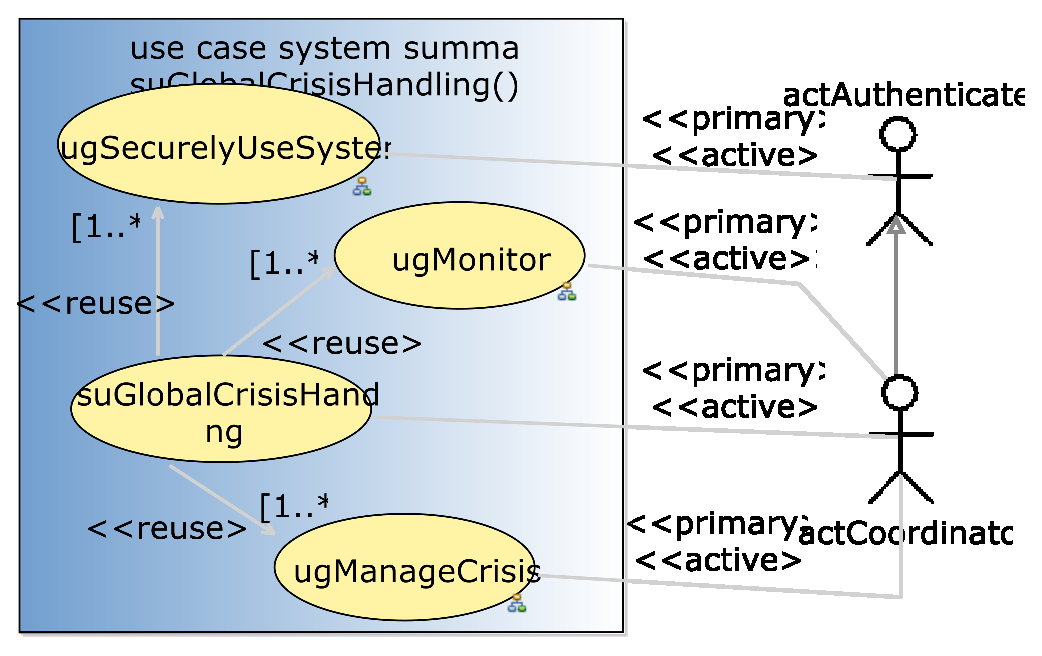
\includegraphics[
angle=0
,scale=0.75
]{./images-report-gen/usecase-model/summary/uc-suGlobalCrisisHandling.eps}
\end{center}
\caption[lu.uni.lassy.excalibur.examples.icrash Use Case Diagram: uc-suGlobalCrisisHandling]{ suGlobalCrisisHandling user goal use case}
\label{fig:lu.uni.lassy.excalibur.examples.icrash-RE-UCD-uc-suGlobalCrisisHandling}
\end{figure}
\vspace{0.5cm}
